\documentclass[nooutcomes]{ximera}
%% handout
%% space
%% newpage
%% numbers
%% nooutcomes



%\begin{image}
%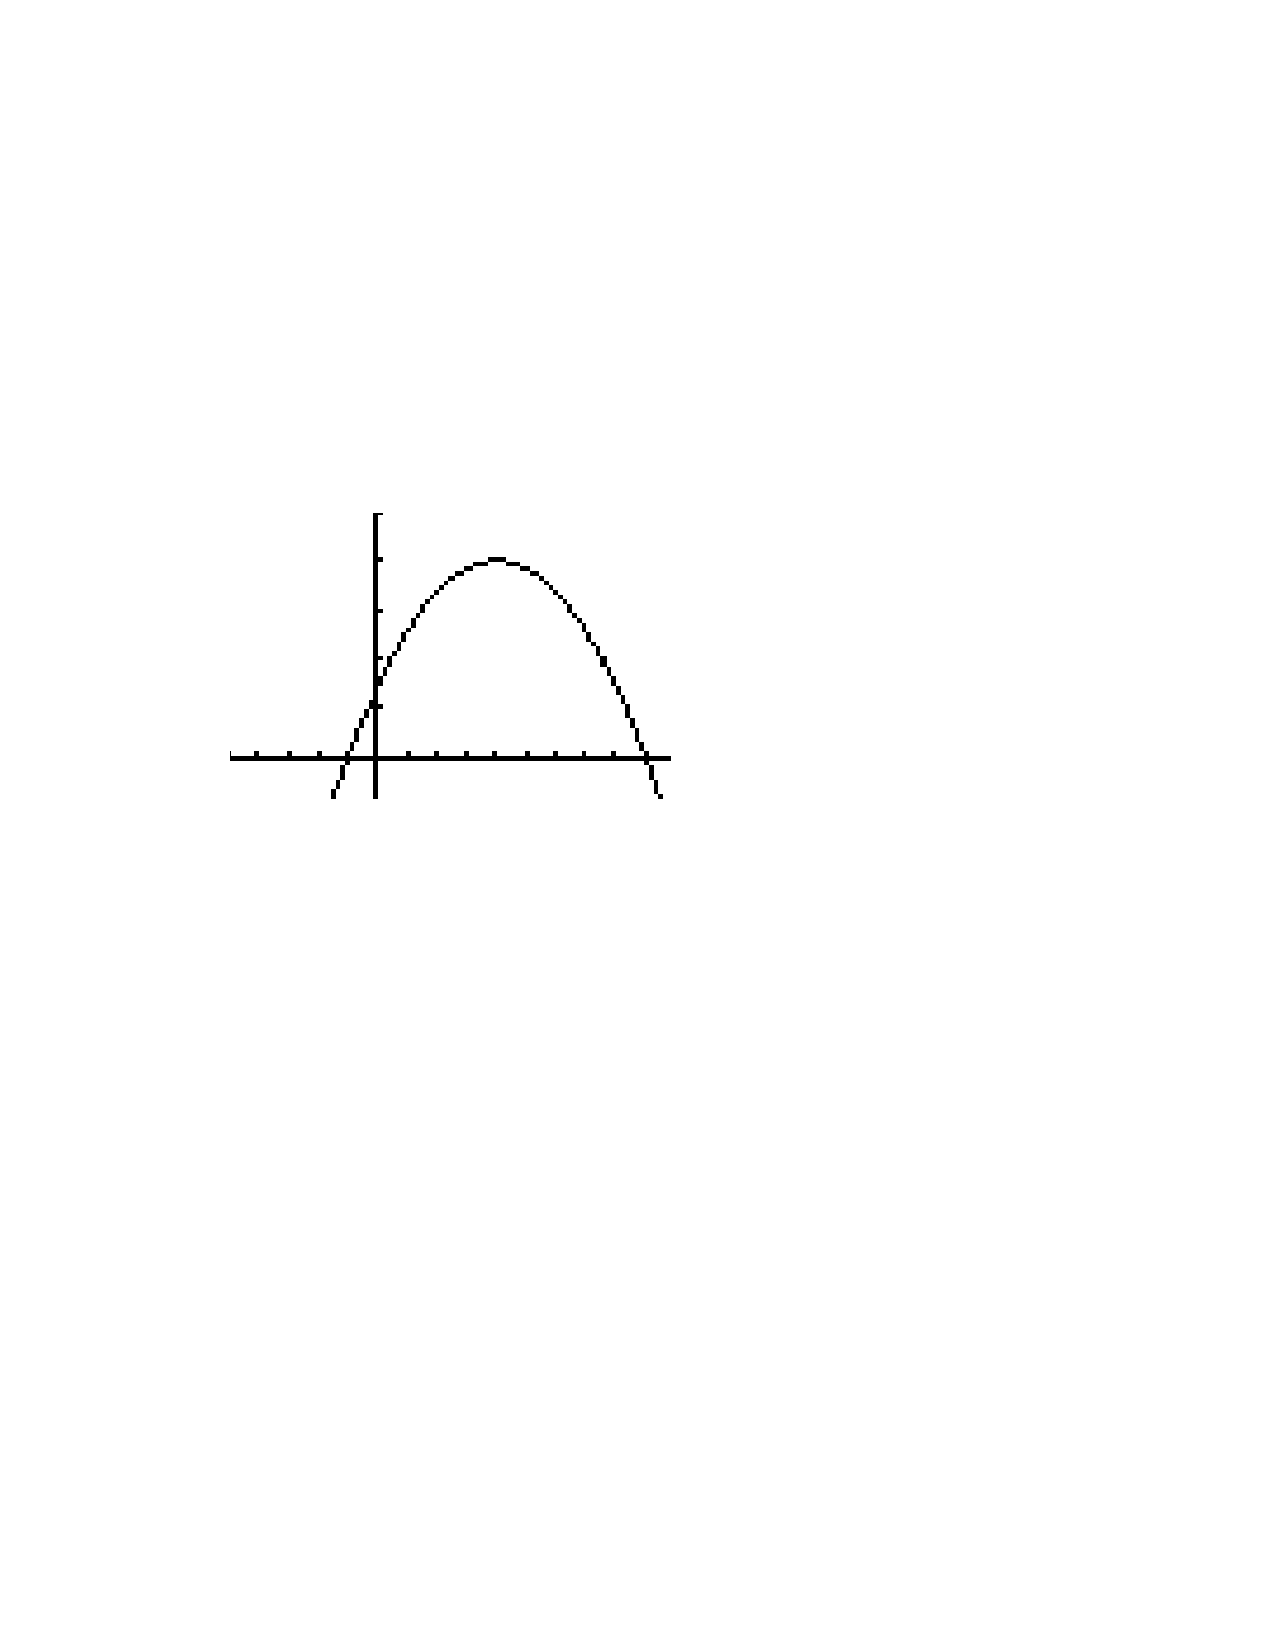
\includegraphics[trim= 170 420 250 180]{Figure1.pdf}
%\end{image}

\usepackage{fullpage}
\newcommand{\RR}{\mathbb R}
\renewcommand{\d}{\,d}
\newcommand{\dd}[2][]{\frac{d #1}{d #2}}
\renewcommand{\l}{\ell}
\newcommand{\ddx}{\frac{d}{dx}}
\newcommand{\dfn}{\textbf}
\newcommand{\eval}[1]{\bigg[ #1 \bigg]}

\usepackage{multicol}

\renewenvironment{freeResponse}{
\ifhandout\setbox0\vbox\bgroup\else
\begin{trivlist}\item[\hskip \labelsep\bfseries Solution:\hspace{2ex}]
\fi}
{\ifhandout\egroup\else
\end{trivlist}
\fi} %% we can turn off input when making a master document

\title{3.11 Related Rates}  

\begin{document}
\begin{abstract}		\end{abstract}
\maketitle


%problem1
\begin{problem}
The radius of a circle is increasing at a rate of 2 inches per minute. 
	\begin{image}
	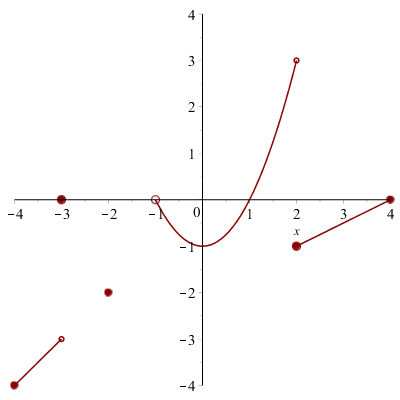
\includegraphics[scale=.5]{Figure2.png}
	\end{image}

\begin{enumerate}
	\item At what rate is the circumference of the circle changing when the radius is 10 inches?
	\begin{freeResponse}
	We know: ${\frac{dr}{dt}}=2$ inches per minute and we want to find ${\frac{dc}{dt}}$ when $r=10$.\\\\
	\begin{align*}
	c&=2\pi r\\
	{\frac{dc}{dt}}&=2\pi {\frac{dr}{dt}}\\
	\eval{{\frac{dc}{dt}}}_{r=10}&=2 \pi (2)\\
	\eval{{\frac{dc}{dt}}}_{r=10}&=4 \pi\ \text{inches per minute}
	\end{align*}
	\end{freeResponse}
	\item At what rate is the area of the circle changing when the radius is 12 inches?
		\begin{freeResponse}
	We know: ${\frac{dr}{dt}}=2$ inches per minute and we want to find ${\frac{dA}{dt}}$ when $r=12$.\\\\
	\begin{align*}
	A&=\pi r^2\\
	{\frac{dA}{dt}}&=2\pi r{\frac{dr}{dt}}\\
	\eval{{\frac{dA}{dt}}}_{r=12}&=2 \pi (12)(2)\\
	\eval{{\frac{dA}{dt}}}_{r=12}&=48 \pi\ \text{inches squared per minute}
	\end{align*}
	\end{freeResponse}
\end{enumerate}

\end{problem}




%problem2
\begin{problem}
Find the mistake in the solution to the given problem.  Then solve the problem correctly.

Two boats leave from the same dock, but at slightly different times.  One boat is traveling east at 30mph while the other boat is traveling north at 15mph.  At an instant in time when the boat traveling east is 15 miles from the dock and the boat traveling north is 10 miles away from the dock, at what rate is the distance between the boats changing?
	\begin{image}
	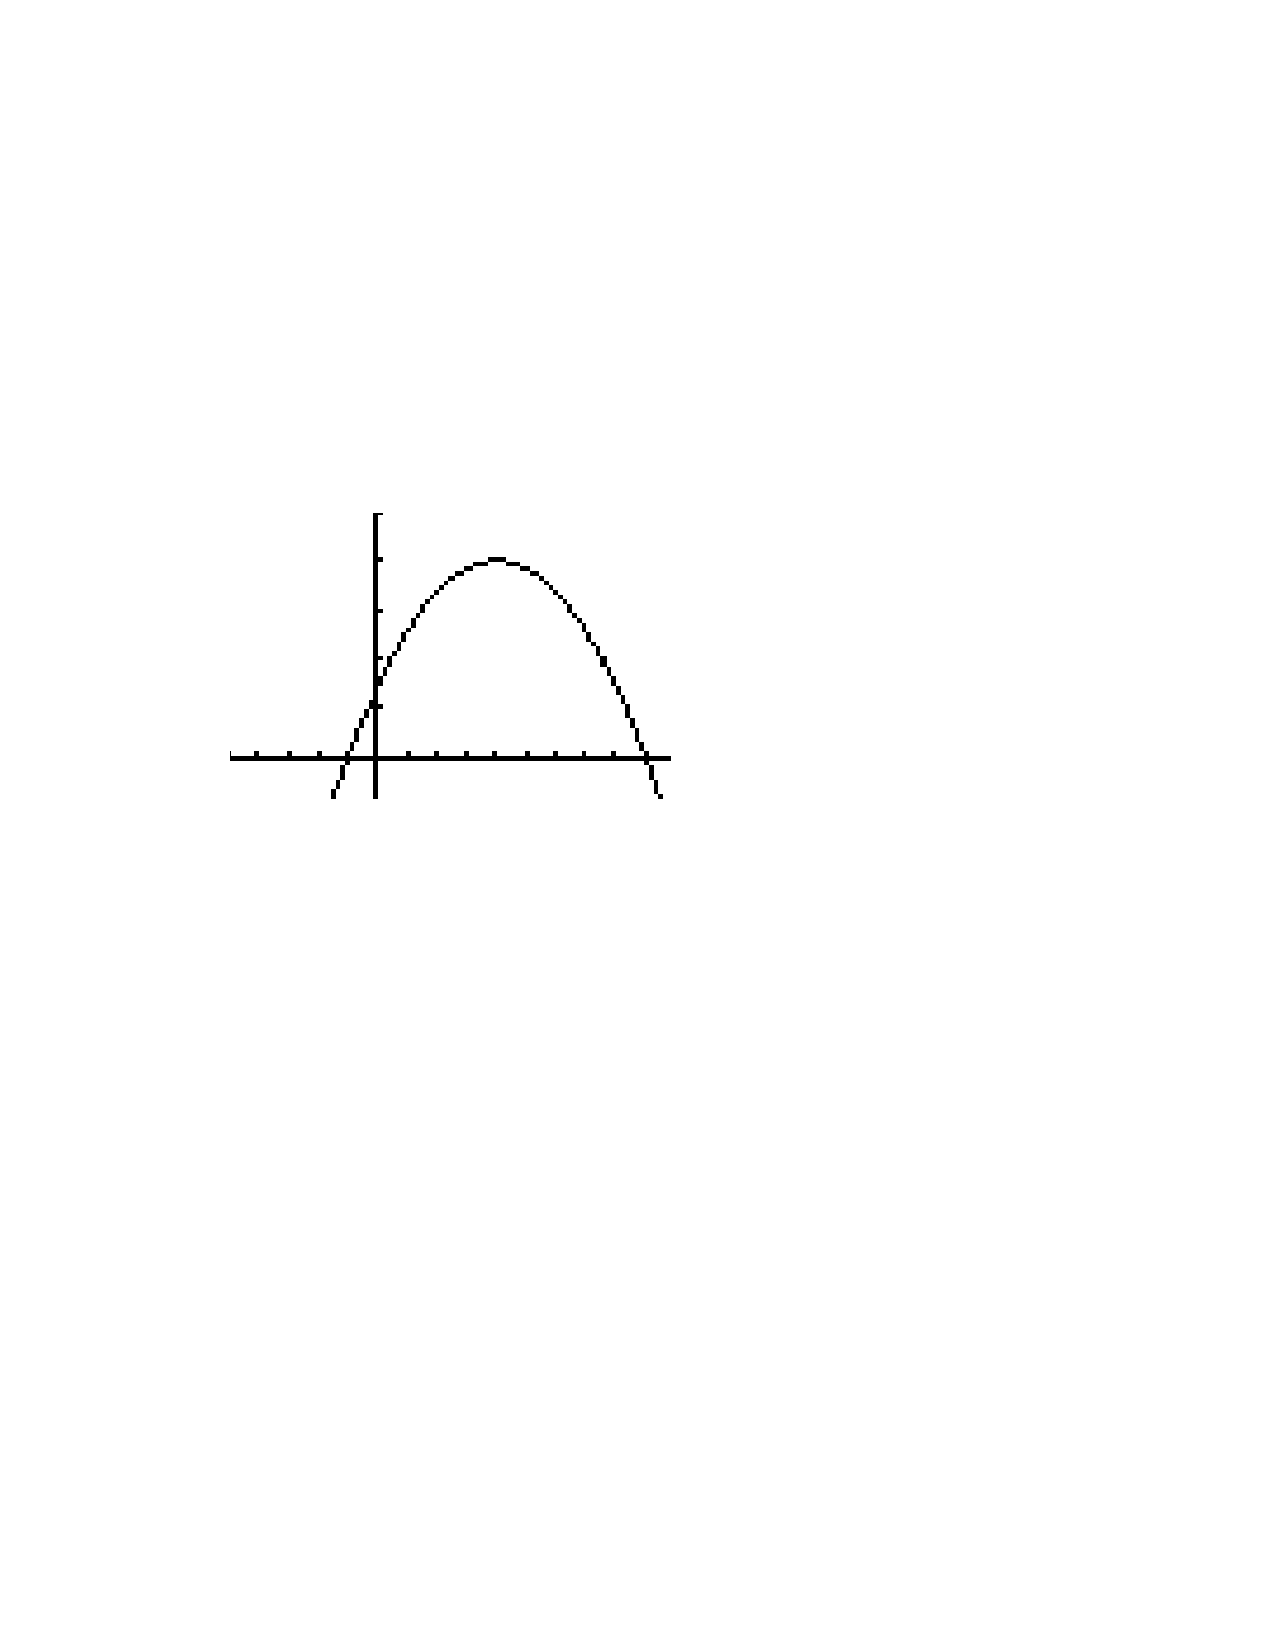
\includegraphics[scale=.7]{Figure1.png}
	\end{image}
	
		\begin{freeResponse} 
		The error occurs when the student plugs in values for $x$ and $y$ \dfn{before} differentiating the equation $x^2 + y^2 = z^2$ with respect to time.  The distances $x$ and $y$ are clearly changing with respect to time, and so they cannot be treated as constants when we are differentiating.
		
		Differentiating $x^2 + y^2 = z^2$ with respect to $t$ yields:
		$$ 2x \dd[x]{t} + 2y \dd[y]{t} = 2z \dd[z]{t}$$
		
		Canceling the 2's and plugging in the known quantities yields:
		$$ z \dd[z]{t} = (15)(30) + (10)(15) = 450 + 150 = 600 $$
		
		In the above work, the student did correctly compute that $z^2 = 325$ at this fixed instant in time.  So $z = 5\sqrt{13}$, and we can solve for $\dd[z]{t}$ to obtain
		$$ \dd[z]{t} = \frac{600}{5 \sqrt{13}} = \frac{120}{\sqrt{13}} \, mph $$
		\end{freeResponse}	

\end{problem}

%problem3
\begin{problem}
A plane flying horizontally at an altitude of 2000 m and a speed of 200 m/sec passes directly over a radar station.  (See figure below.)  Find the rate at which the distance from the plane to the station is increasing 5 seconds after the plane passed directly over the radar station.  Make sure to label the figure.

	\begin{image}
	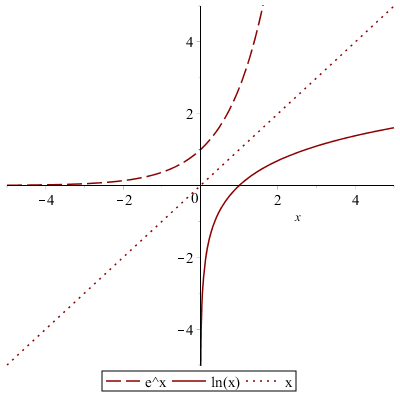
\includegraphics[scale=.5]{Figure4.png}
	\end{image}
\begin{freeResponse} \hfil

	\begin{image}
	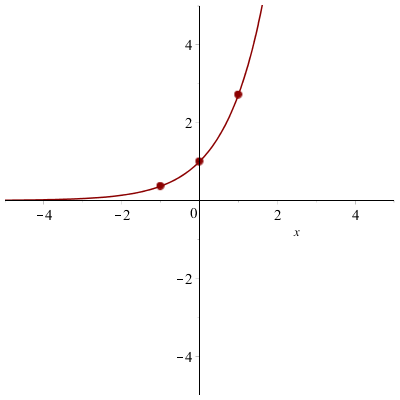
\includegraphics[scale=.5]{Figure5.png}
	\end{image}

	\begin{align*}
	y^2&=2000^2+x^2\\
	2y{\frac{dy}{dt}}&=2x{\frac{dx}{dt}}\ \text{(see $x$ and $y$ solved below)}\\
	\sqrt{1000^2+2000^2}\eval{{\frac{dy}{dt}}}_{t=5}&=1000 \cdot 200 \\
	\eval{{\frac{dy}{dt}}}_{t=5}&=\frac{1000 \cdot 200}{\sqrt{1000^2+2000^2}}\ \text{m/s}
	\end{align*}

Solving for $x$ when $t=5$:\\
We use the distance formula.  Distance=rate*time, $d=rt$.  Here we have $x=rt$.  $x=(5)(200)=1000$\ m  \\\\

Solving for $y$ when $t=5$:
	\begin{image}
	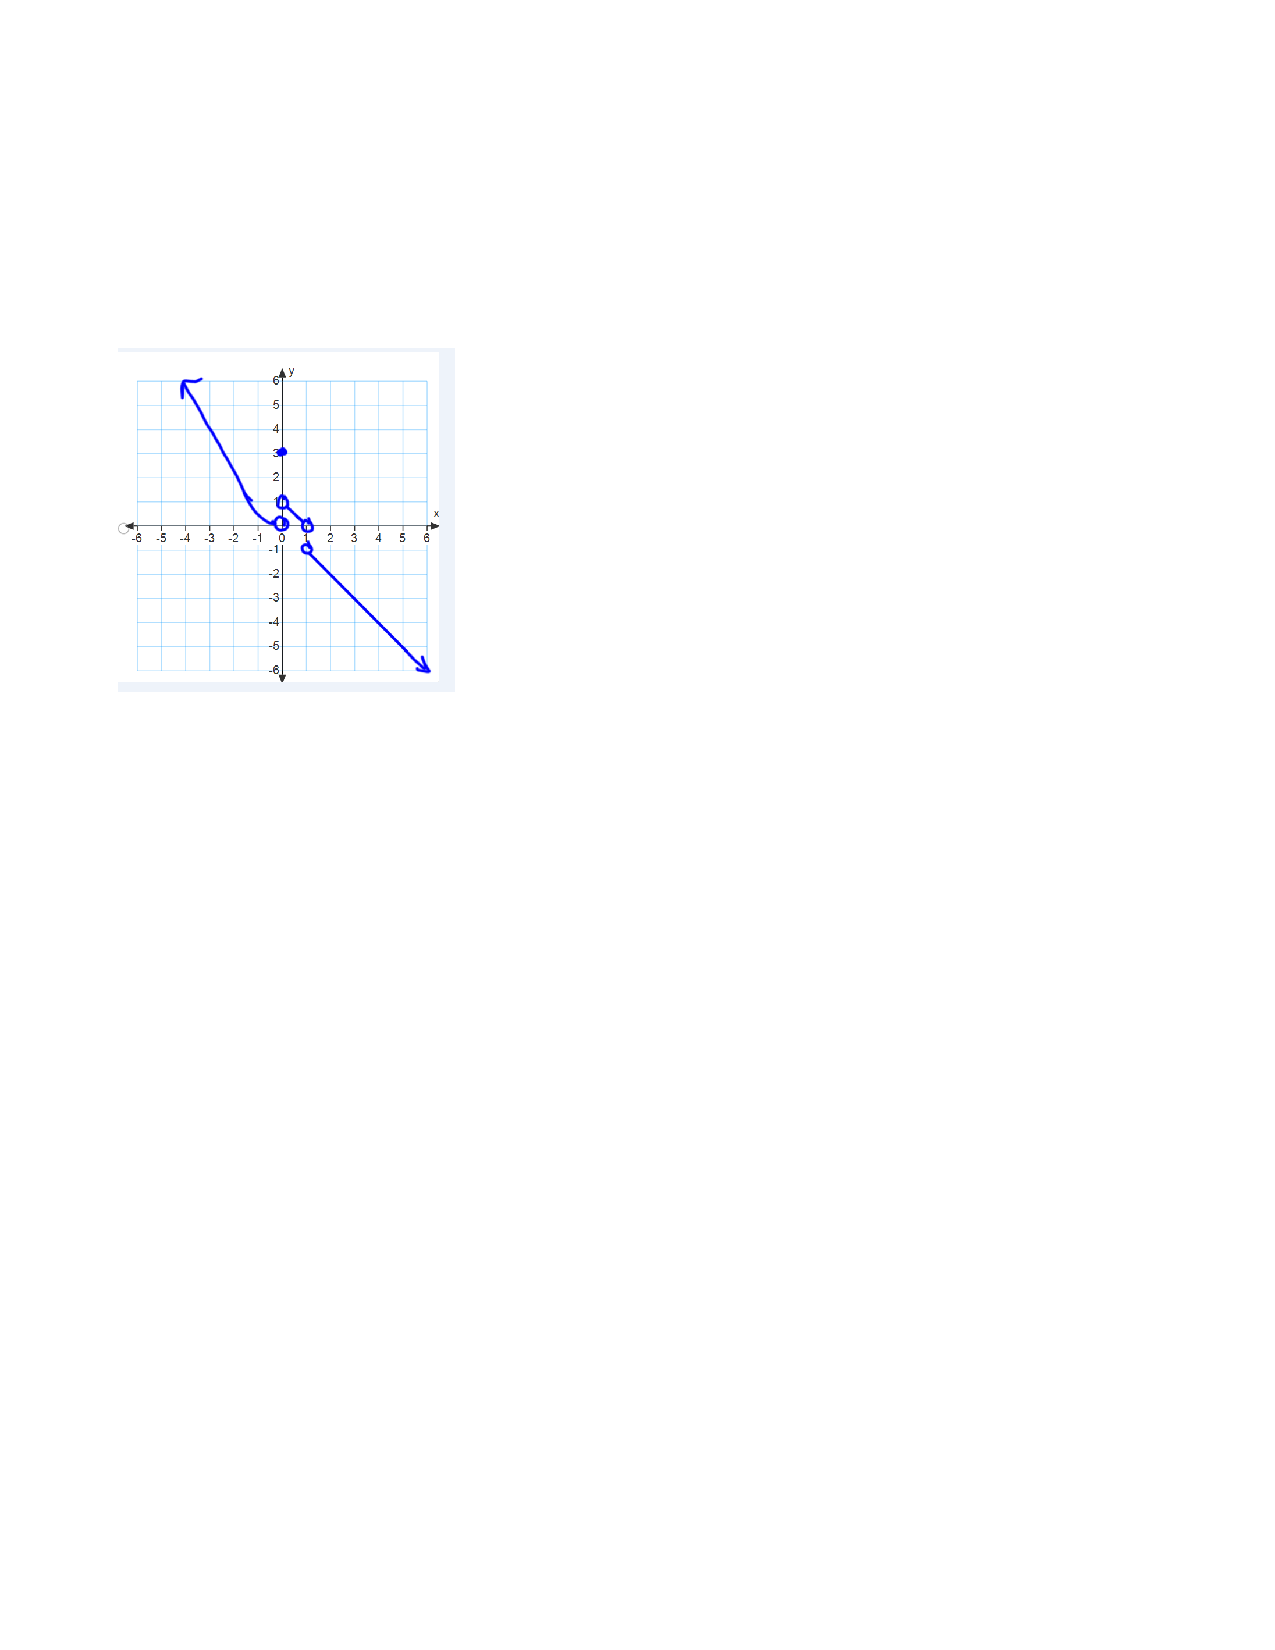
\includegraphics[scale=.5]{Figure3.png}
	\end{image}

\end{freeResponse}
\end{problem}

%problem4
\begin{problem}
A plane flying horizontally at an altitude of 800m and speed of 200 m/sec passes directly over a spectator at an air show. (See figure below.)  Find the rate at which the angle of elevation, $\theta$, is changing 4 seconds later. Make sure to label the figure. ($\theta =$\ angle between the ground and the line from the spectator to the plane)   

	\begin{image}
	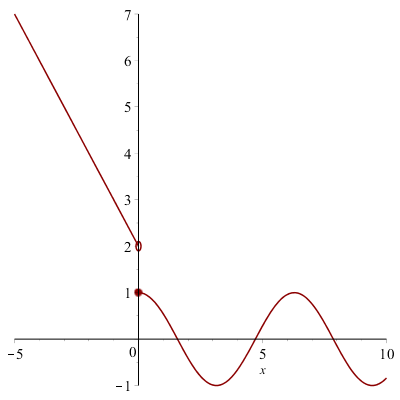
\includegraphics[scale=.5]{Figure6.png}
	\end{image}
\begin{freeResponse} \hfil
	\begin{image}
	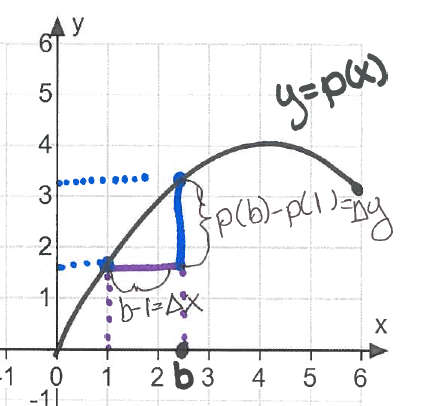
\includegraphics[scale=.3]{Figure7.png}
	\end{image}

	\begin{align*}
	\tan {\theta}&=\frac{800}{x}\\
	\sec^2{\theta} \cdot \frac{d\theta}{dt}&=\frac{-800}{x^2}\cdot \frac{dx}{dt}\ \text{(see $x$ and $\sec(\theta)$ solved below)}\\
	2 \cdot \eval{\frac{d\theta}{dt}}_{t=4}&=\frac{-800}{800^2}\cdot 200  \\
	\eval{\frac{d\theta}{dt}}_{t=4}&=\frac{-800}{800^2}\cdot 200 \cdot \frac{1}{2}=-\frac{1}{8} \text{radians per second}
	\end{align*}

To solve for $x$ when $t=4$:\\
Use $d=rt$.  Here we have $x=rt$.  $x=(200)(4)=800$\ m  \\\\

To solve for $\sec{\theta}$ when $t=4$:\\
Since the two legs of the triangle are equal, $\theta=\frac{\pi}{4}$\\
$\cos\left({\frac{\pi}{4}}\right)=\frac{1}{\sqrt{2}} \implies \sec\left({\frac{\pi}{4}}\right)=\sqrt{2}$





\end{freeResponse}
\end{problem}

%problem5
\begin{problem}
A ciylindrical swimming pool with a radius of 10 feet and height of 5 feet is being filled with water.  How fast is the water being pumped into the pool (in ft$^3$/min) if the water level is increasing at a rate of 6 in/minute?  Make sure to draw a picture to represent the situation.
\begin{freeResponse} \hfil
	\begin{image}
	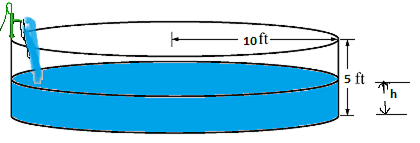
\includegraphics[scale=.7]{Figure18.png}
	\end{image}
	
	
	\begin{align*}
	\frac{dh}{dt}&=6 \text{in/min}=.5 \text{feet/min}\\
	V&=\pi r^2h=\pi(100)h \\
	\frac{dV}{dt}&=100\pi \frac{dh}{dt}\\
	\frac{dV}{dt}&=100 \pi (.5)=50 \pi \text{ft}^3\text{/min}
	\end{align*}


\end{freeResponse}
	
	
\end{problem}


%problem6
\begin{problem}
A part of a circle centered at the origin with radius $r=7$ cm is given in the figure (A) below.  A right triangle is formed in the first quadrant (see Figure (A)).  One of its sides lies on the x-axis.  Its hypotenuse runs from the origin to a point on the circle.  The hypotenuse makes an angle $\theta$ with the x-axis.  Assume that the angle $\theta$ changes at the rate $\frac{d\theta}{dt}=0.2$\ radians per second.
	\begin{image}
	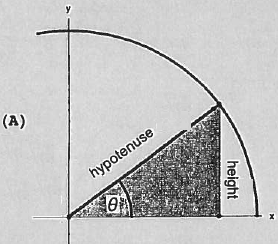
\includegraphics[scale=.5]{Figure10.png}
	\end{image}
	
\begin{enumerate}
	\item Label Figure A.
		\begin{freeResponse} \hfil
		\begin{image}
	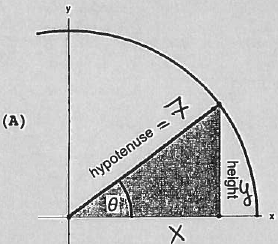
\includegraphics[scale=.5]{Figure11.png}
	\end{image}
		\end{freeResponse}
	\item In Figure B, draw the the triangle twice; once when $\theta$ is small and once more, when $\theta$ is close to $\frac{\pi}{2}$.

		\begin{image}
	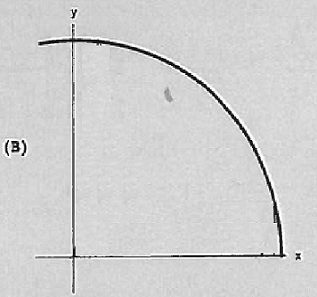
\includegraphics[scale=.4]{Figure12.png}
	\end{image}
		\begin{freeResponse} \hfil
		\begin{image}
		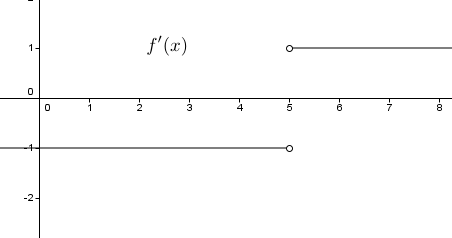
\includegraphics[scale=.5]{Figure13.png}
		\end{image}
		\end{freeResponse}
	\item Find the rate of change of the height of the triangle when $\theta=\frac{\pi}{3}$
		\begin{freeResponse}
		$y=7\sin{\theta}$
		\begin{align*}
		\frac{dy}{dt}&=\frac{dy}{d\theta}\cdot \frac{d\theta}{dt}\\
		\frac{dy}{dt}&=7\cos{\theta} \cdot \frac{d\theta}{dt}\\
		\eval{\frac{dy}{dt}}_{\theta=\frac{\pi}{3}}&=7(1/2)(0.2)\\
		&=0.7 \text{cm/sec}
		\end{align*}
				\end{freeResponse}
	\item Find the rate of change of the area of the triangle when $\theta=\frac{\pi}{3}$
		\begin{freeResponse}
		First, we need to find $x$: $x=7 \cos{\theta}$.  From part c, we know $y=7\sin{\theta}$
		\begin{align*}
		A&=\frac{1}{2}xy\\
		A&=\frac{49}{2}\cos(\theta)\sin(\theta)\\
		\frac{dA}{dt}&=\frac{49}{2}(-\sin^2(\theta)+\cos^2(\theta)) \cdot \frac{d\theta}{dt}\\
		\eval{\frac{dA}{dt}}_{\theta=\frac{\pi}{3}}&=\frac{49}{2}\left(-\left(\frac{\sqrt{3}}{2}\right)^2+\left(\frac{1}{2}\right)^2 \right) \cdot 0.2\\\\
		&=\frac{49}{2}\cdot \frac{-1}{2} \cdot 0.2\\
		&=\frac{-4.9}{2} cm^2/sec
		\end{align*}
		\end{freeResponse}
\end{enumerate}
\end{problem}

%problem7
\begin{problem}
A conical water tank of height 10 feet and radius 4 feet is being drained through a hole in the bottom (See figure below).   
		\begin{image}
		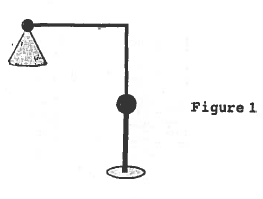
\includegraphics[scale=.4]{Figure14.png}
		\end{image}

\begin{enumerate}
	\item Let $r$ be the radius of the water at depth $h$.  In the figure above, label $r$ and $h$.
		\begin{freeResponse} \hfil
		\begin{image}
		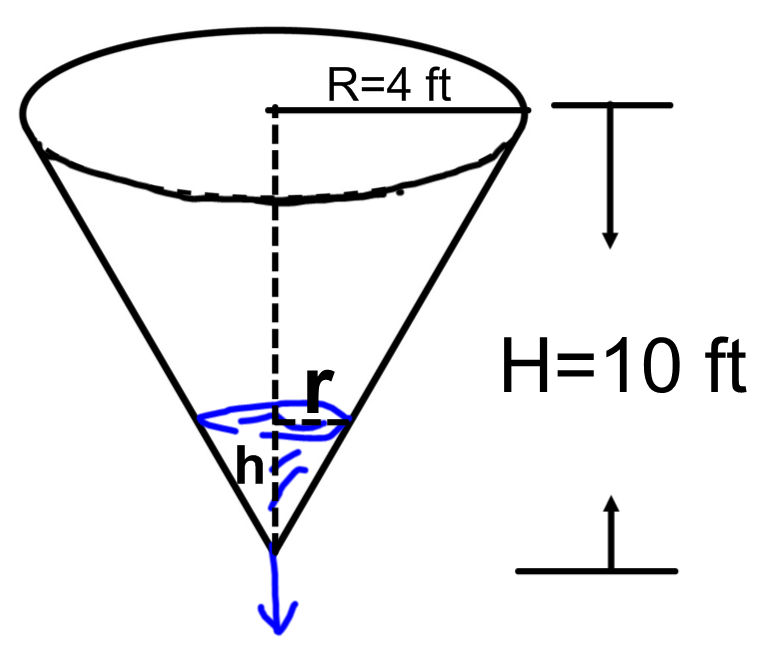
\includegraphics[scale=.4]{Figure15.png}
		\end{image}
		\end{freeResponse}	
	\item Find an expression for $r$ in terms of $r$.
	$\frac{r}{h}=\frac{R}{H}=\frac{4}{10}=\frac{2}{5} \implies r=\frac{2}{5}h$
	
	\item The water in the tank is being drained at a rate of 2 feet$^3$ per minute.  What is the rate of change of the water depth when the water dept is 1 foot?

	\begin{freeResponse}
	Let $V$ be volume of water in the tank.  We were given $\frac{dV}{dt}=2$ feet$^3$/min. \\
	We can relate the volume of water in the tank to the water height by the formula for the volume of a cone: $V=\frac{1}{3}\pi r^2 h$. \\\\
	We have already found $r$ in terms of $h$ so subsituting gives us:  $V=\frac{1}{3}\pi \left(\frac{2}{5}h\right)^2\cdot h=\frac{4}{75}\pi h^3$
	
	\begin{align*}
	V&=\frac{4}{75}\pi h^3\\
	\frac{dV}{dt}&=\frac{4}{75}\pi \cdot 3h^2 \cdot \frac{dh}{dt} \\
	\frac{dV}{dt}&=\frac{4}{25}\pi h^2 \cdot \frac{dh}{dt} \\
	-2&=\frac{4}{25}\pi (3)^2 \cdot \eval{\frac{dh}{dt}}_{h=3} \\
	\eval{\frac{dh}{dt}}_{h=3}&=-\frac{25}{18 \pi} ft/sec
	\end{align*}


\end{freeResponse}
\end{enumerate}
\end{problem}


%problem8
\begin{problem}
A right cone has a fixed slant height (see figure below) of 9 ft.  The cone's height is shrinking at a rate of 0.5 ft/sec.  At what rate is the area of the base changing when the height is 6 ft?  Be sure to label the picture.
	\begin{image}
	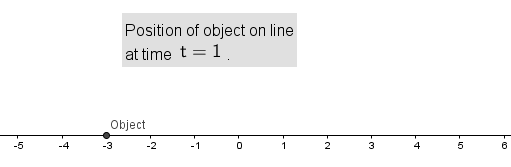
\includegraphics[scale=.5]{Figure8.png}
	\end{image}
\begin{freeResponse}
	\begin{image}
	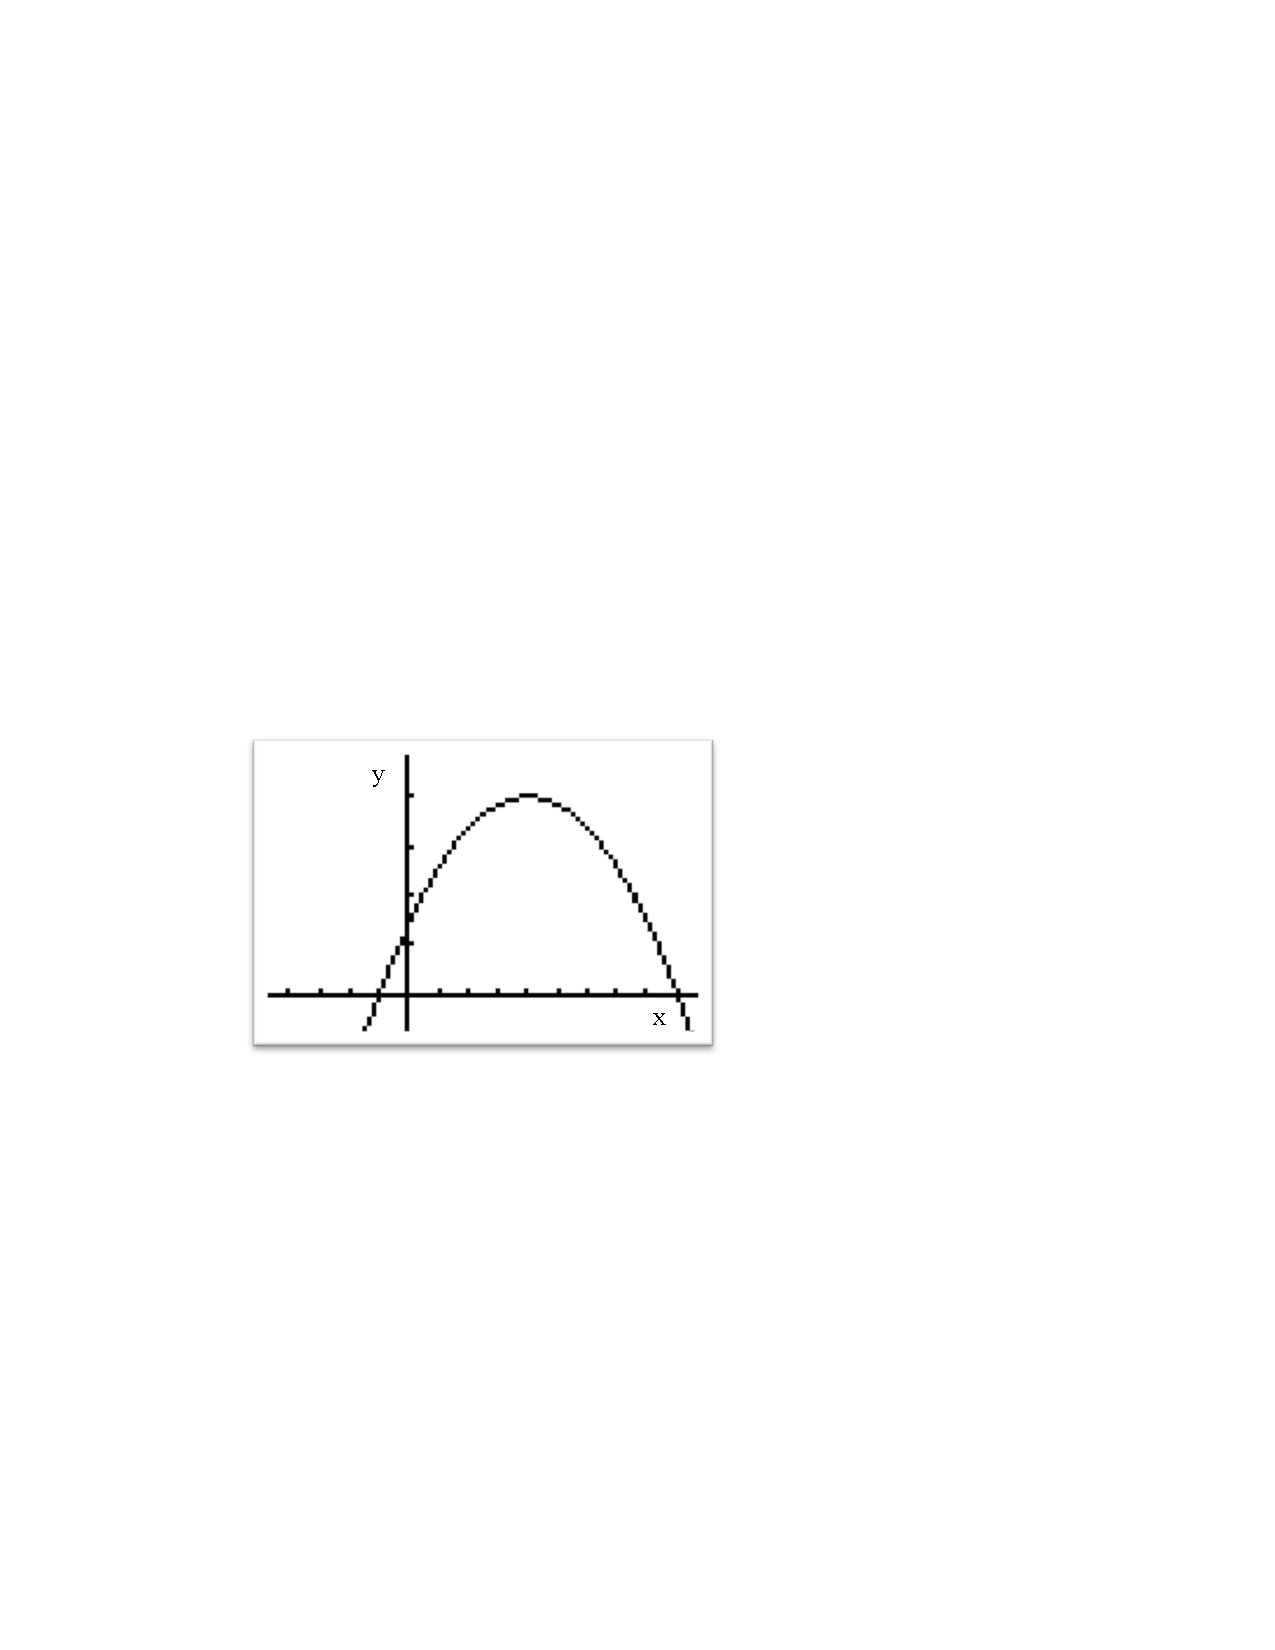
\includegraphics[scale=.5]{Figure9.png}
	\end{image}

	\begin{align*}
	A&=r^2\pi\\
	\frac{dA}{dt}&=2r\pi \cdot \frac{dr}{dt} 
	\end{align*}
	We don't know $r$ or $\frac{dr}{dt}$ so we need to relate these to $h$ and $\frac{dh}{dt}$ which we do know:\\
	\begin{align*}
	r^2+h^2&=9^2\\
	2r\frac{dr}{dt}+2h\frac{dh}{dt}&=0\\
	2r\frac{dr}{dt}&=-2h\frac{dh}{dt}\\
	\text{so we have:}&\\
	\frac{dA}{dt}&=-2h\pi \cdot \frac{dh}{dt} \\
	\eval{\frac{dA}{dt}}_{t=6}&=-2(6)\pi (-.05)\\
	\eval{\frac{dA}{dt}}_{t=6}&=6\pi \text{feet squared per second}
	\end{align*}

\end{freeResponse}
\end{problem}


\end{document} 


















